\section{连续型随机变量及其分布函数}

\subsection{分布律与分布函数}
对于一个连续型随机变量$X$,由于其可能取的值不能一一列举出来,因而就不能像离散型随机变量那样可以用分布律来描述,这是因为,我们无法说连续型随机变量的在某一个值上的概率是多少。试想以$X$表示某个灯泡的寿命小时数,我们没办法去说$X$为$1,2,3,\cdots$的概率是多少,介于$X$还有$1.01,1.002,\sqrt{2},e/2,\pi/2$等太多值可以取,换言之,\empx{连续型随机变量在任何一个值上的概率都是零}。但是,仍有一样东西是可以研究的,例如,我们可以去讨论灯泡的寿命小时数$X$落在区间$(0,1], (1,2], (2,3]$的概率是多少,一般的说,即$P\qty{x_1<X\leq x_2}$。

但是,由于$P\qty{x_1<X\leq x_2}$,显然可以表示为
\begin{Equation}
    P\qty{x_1<X\leq x_2}=P\qty{x\leq x_2}-P\qty{X\leq x_1}
\end{Equation}
所以我们只需要研究随机变量小于等于某个值的概率就可以了,由此,引入分布函数。
\begin{BoxDefinition}[分布函数]
    设$X$是一个随机变量,而$x$是任意实数,则定义函数
    \begin{Equation}
        F(x)=P\qty{X\leq x},\qquad -\infty<x<\infty
    \end{Equation}
    称为$X$的\uwave{分布函数}或\uwave{累积分布函数}(Cumulative Distribution Function,CDF)。
\end{BoxDefinition}

简单来说,分布函数$F(x)$即表示随机变量$X$落在区间$(-\infty,x]$的概率。

\begin{BoxProperty}[分布函数的不减性]
    分布函数$F(x)$是一个不减函数,换言之,对于$\forall x_1,x_2\in\R$,若$x_2>x_1$
    \begin{Equation}
        F(x_2)\geq F(x_1)
    \end{Equation}
\end{BoxProperty}
\begin{Proof}
    这是很显然的,如果$x_2>x_1$,那么$(-\infty,x_2]$是包含$(-\infty,x_1]$且更大的一个区间,而随机变量$X$落在$(-\infty,x_2]$的概率显然大于落在其子区间$(-\infty,x_1]$的概率,故$F(x_2)\geq F(x_1)$。
\end{Proof}

\begin{BoxProperty}[分布函数的极限]
    分布函数$F(x)$在无穷大处的极限为
    \begin{Equation}
        F(-\infty)=0\qquad F(+\infty)=1
    \end{Equation}
\end{BoxProperty}
\begin{Proof}
    这亦是显然的,因为$F(-\infty)$是不可能事件,而$F(+\infty)$是必然事件。
\end{Proof}

\begin{BoxProperty}[分布函数的右连续]
    分布函数$F(x)$满足右连续性
    \begin{Equation}
        F(x+0)=F(x)
    \end{Equation}
\end{BoxProperty}

\begin{Proof}
    证明从略。
\end{Proof}


需要指出的是,虽然分布函数是为连续性随机变量准备的概念,但是分布函数其实也完全可以适用于离散型随机变量,尽管分布律已经可以全面描述离散型随机变量。例如,若有分布律
\begin{Equation}
    f(x)=
    \begin{cases}
        0.2,&x=0\\
        0.3,&x=1\\
        0.5,&x=2\\
    \end{cases}
\end{Equation}
那么,相应的分布函数就是
\begin{Equation}
    F(x)=
    \begin{cases}
        0.0,&x\leq 0\\
        0.2,&0<x\leq 1\\
        0.5,&1<x\leq 2\\
        1.0,&x>2
    \end{cases}
\end{Equation}
由此可见,离散型随机变量的分布函数就是一个分段的阶梯函数。

\subsection{概率与概率密度}
我们知道,分布律描述的是随机变量落在$x$处的概率,这种想法仅适用于离散型随机变量,却无法适用于连续性随机变量。分布函数描述的则是随机变量落在$-\infty$至$x$间的概率,这对于连续性随机变量是有值的,但问题是,我还是更关心“在某一个点附近的概率状况”。为此,我们可以将分布函数视为某个函数的积分,或者说,我们试图找到分布函数的导函数,它能表征在$x$附近概率的变化率,这就是概率密度。下面,我们用数学化的语言正式定义概率密度。

\begin{BoxDefinition}[概率密度]
    若对于随机变量$X$的分布函数$F(x)$,存在非负可积函数$f(x)$,对于任意的$x$,有
    \begin{Equation}
        F(x)=\Int[-\infty][x]f(\xi)\dd{\xi}
    \end{Equation}
    那么,就称随机变量$X$为连续性随机变量。
    
    函数$f(x)$称为$X$的\uwave{概率密度函数}(Probability Density Function),简称\uwave{概率密度}。
\end{BoxDefinition}
我们知道,分布函数可以统一的描述离散型随机变量和连续性随机变量的概率分布特征,而这里\xref{def:概率密度}告诉我们,通过分布函数是否存在概率密度函数,可以区分随机变量的类型
\begin{itemize}
    \item 离散型随机变量的分布函数是分段的,无法定义概率密度函数,只能定义分布律。
    \item 连续型随机变量的分布函数是连续的,可以定义概率密度函数。\footnote{这里的提法不太严谨,实际上存在非离散但也并不连续的随机变量,但这不是我们要考虑的。}
\end{itemize}
我们可以这样去理解,离散型随机变量的分布律对应连续性随机变量的概率密度函数,这是因为,前者描述的是在每个离散点的概率,后者描述的是在每个连续点的概率密度。引入分布函数的主要目的,就是统一离散型随机变量和连续性随机变量,并由此导出概率密度的概念。

\begin{BoxProperty}[概率密度的非负性]
    概率密度$f(x)$具有非负性
    \begin{Equation}
        f(x)\geq 0
    \end{Equation}
\end{BoxProperty}
\begin{Proof}
    由\fancyref{ppt:分布函数的不减性}可以立即得到。
\end{Proof}\goodbreak

\begin{BoxProperty}[概率密度的归一性]
    概率密度$f(x)$具有归一性
    \begin{Equation}
        \Int[-\infty][\infty]f(x)\dx=1
    \end{Equation}
\end{BoxProperty}\nopagebreak
\begin{Proof}
    显然,概率的总和是$1$,由\fancyref{ppt:分布函数的极限}和\fancyref{def:概率密度}可得。
\end{Proof}

\begin{BoxProperty}[概率密度与概率]
    概率密度$f(x)$在区间上的积分即该区间上的概率
    \begin{Equation}
        \Int[a][b]f(x)\dx=F(b)-F(a)
    \end{Equation}
    其中$F(x)$是随机变量分布函数。
\end{BoxProperty}
\begin{Proof}
    显然,概率是概率密度的积分,由\fancyref{def:概率密度}可得。
\end{Proof}

值得注意的是,\empx{概率为零并非不可能事件},连续性随机变量就是这一事实的反例,尽管,连续性随机变量在任何一个特定取值处的概率都是零,但是,从连续性随机变量的概率密度函数看,这些取值并非是不可能出现的,即对于连续性随机变量,\empx{概率密度为零才是不可能事件}。

\subsection{均匀分布}
\begin{BoxDefinition}[均匀分布]
    若连续性随机变量$X$具有概率密度
    \begin{Equation}
        f(x)=
        \begin{cases}
            \mal{\frac{1}{b-a}}&{a<x<b}\\[3mm]
            0&\text{otherwise}
        \end{cases}
    \end{Equation}
    则称$X$在区间$(a,b)$上服从\uwave{均匀分布}(Uniform Distribution),记为
    \begin{Equation}
        X\sim U(a,b)
    \end{Equation}
\end{BoxDefinition}

均匀分布的特征是等可能性,具体而言,如果随机变量$X$服从均匀分布$U(a,b)$,那么$X$落在区间$(a,b)$中任意等长度的子区间内的可能性是相同的。换言之,服从均匀分布$U(a,b)$的随机变量,其落在$(a,b)$的某个子区间的概率,只依赖子区间的长度,而与子区间的位置无关。

均匀分布函数显然满足归一性,并且,其分布函数也是容易求出的,这是常数的积分。
\begin{BoxFormula}[均匀分布的分布函数]
    若$X$服从均匀分布$U(a,b)$,则其分布函数为
    \begin{Equation}
        F(x)=
        \begin{cases}
            0,&x<a\\[3mm]
            \mal{\frac{x-a}{b-a}},&a\leq x<b\\[3mm]
            1,&x\leq b    
        \end{cases}
    \end{Equation}
\end{BoxFormula}
\begin{Proof}
    当$x<a$或$x\geq b$时$F(x)=0,1$是显然的,当$a\leq x<b$时
    \begin{Equation}*
        F(x)=\Int[-\infty][x]f(\xi)\dx=\Int[a][x]f(\xi)\dd{\xi}=\Int[a][x]\frac{1}{b-a}\dd{\xi}=\frac{x-a}{b-a}\qedhere
    \end{Equation}
\end{Proof}

\subsection{指数分布}
\begin{BoxDefinition}[指数分布]
    若连续性随机变量$X$具有概率密度
    \begin{Equation}
        f(x)=
        \begin{cases}
            \mal{\frac{1}{\theta}\exp(-\frac{x}{\theta})},& x>0\\[3mm]
            0,& \text{otherwise}
        \end{cases}
    \end{Equation}
    则称$X$服从参数为$\theta$的\uwave{指数分布}(Exponential Distribution),记为
    \begin{Equation}
        X\sim \Exp(\theta)
    \end{Equation}
\end{BoxDefinition}
指数分布的概率密度函数如\xref{fig:指数分布的概率密度}所示(这其实是一个负指数函数),注意到,当指数分布的参数$\theta$越大,则概率密度在$x$较小时会相对比较大,但是随着$x$增大下降的也会越快。

\begin{BoxProperty}[指数分布的归一性]
    指数分布满足归一性要求
    \begin{Equation}
        \Int[0][\infty]\frac{1}{\theta}\exp(-\frac{x}{\theta})\dx=1
    \end{Equation}
\end{BoxProperty}

\begin{Proof}
    这是显然的
    \begin{Equation}*
        \Int[0][\infty]\frac{1}{\theta}\exp(-\frac{x}{\theta})\dx=-\eval{\exp(-\frac{x}{\theta})}_0^{\infty}=1\qedhere
    \end{Equation}
\end{Proof}

\begin{BoxProperty}[指数分布的分布函数]
    指数分布的分布函数为
    \begin{Equation}
        F(x)=\begin{cases}
            \mal{1-\exp(-\frac{x}{\theta})},&x>0\\[3mm]
            0,&\text{otherwise}
        \end{cases}
    \end{Equation}
\end{BoxProperty}

\begin{Proof}
    当$x<0$时$F(x)$显然为零,而对于$x>0$的情况
    \begin{Equation}*
        F(x)=\Int[-\infty][x]f(\xi)\dd{\xi}=\Int[0][x]f(\xi)\dd{\xi}=\Int[0][x]\frac{1}{\theta}\exp(-\frac{\xi}{\theta})\dd{\xi}=\eval{-\exp(-\frac{\xi}{\theta})}_0^{x}=1-\exp(-\frac{x}{\theta})
    \end{Equation}
\end{Proof}

指数分布的分布函数的图像,如\xref{fig:指数分布的分布函数}所示,参数$\theta$越大,趋近$1$的速度越慢。

\begin{Figure}[指数分布]
    \begin{FigureSub}[指数分布的概率密度]
        \hspace{1cm}
        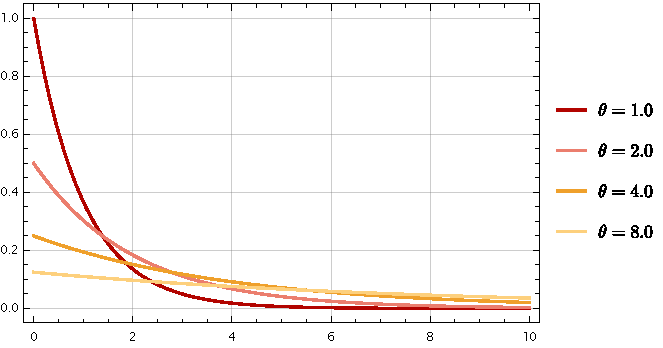
\includegraphics[scale=0.9]{Mathematica/output/ExpFunc.pdf}
    \end{FigureSub}\\ \vspace{0.5cm}
    \begin{FigureSub}[指数分布的分布函数]
        \hspace{1cm}
        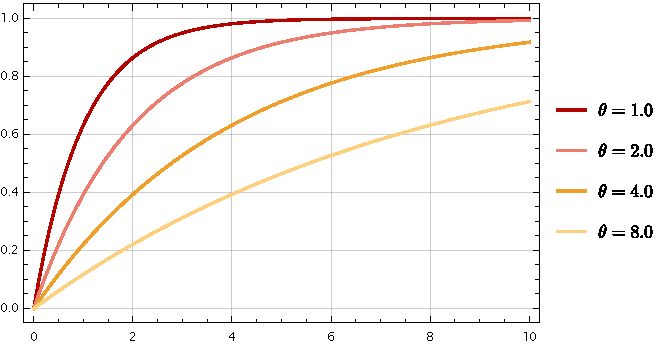
\includegraphics[scale=0.9]{Mathematica/output/ExpFuncF.pdf}
    \end{FigureSub}
\end{Figure}
指数分布有一些有趣的性质。

\begin{BoxProperty}[指数分布的无记忆性]
    指数分布具有无记忆性,即对于任意的$s,t>0$
    \begin{Equation}
        P\qty{x>s+t\mid x>s}=P\qty{x>t}
    \end{Equation}
\end{BoxProperty}

\begin{Proof}
    根据\fancyref{thm:贝叶斯定理}
    \begin{Equation}
        P\qty{x>s+t\mid x>s}=\frac{P\qty{(x>s+t)\cap \qty(x>s)}}{P\qty{x>s}}
    \end{Equation}
    很明显$x>s$和$x>s+t$的交集仍然是后者,因此
    \begin{Equation}
        P\qty{x>s+t\mid x>s}=\frac{P\qty{x>s+t}}{P\qty{x>s}}
    \end{Equation}
    我们可以改用分布函数的表示
    \begin{Equation}
        P\qty{x>s+t\mid x>s}=\frac{1-F(s+t)}{1-F(s)}
    \end{Equation}
    代入\fancyref{ppt:指数分布的分布函数}
    \begin{Equation}*
        P\qty{x>s+t\mid x>s}=\frac{\exp[-(s+t)/\theta]}{\exp(-s/\theta)}=\exp(-t/\theta)=P\qty{X>t}\qedhere
    \end{Equation}
\end{Proof}

试想,通常来说元件的寿命是服从指数分布的,寿命越长的概率越小。由此可见,指数分布的无记忆性的意义是,如果元件已经正常工作了$s$小时,那么,元件能至少继续工作$t$小时的概率与新元件至少正常工作$t$小时的概率是相同的,换言之,元件并不记得自己工作了多久。

\subsection{正态分布}
\begin{BoxDefinition}[正态分布]
    若连续性随机变量$X$具有概率密度
    \begin{Equation}
        f(x)=\frac{1}{\sqrt{2\pi}\sigma}\exp[-\frac{(x-\mu)^2}{2\sigma^2}]
    \end{Equation}
    则称$X$服从参数为$\mu,\sigma$的\uwave{正态分布}(Normal distribution),记为
    \begin{Equation}
        X\sim N(\mu,\sigma^2)
    \end{Equation}
    正态分布亦称为\uwave{高斯分布}(Gaussian Distribution)。
\end{BoxDefinition}\goodbreak
正态分布的概率密度如\xref{fig:正态分布的概率密度}所示,这表现为一个钟形曲线
\begin{itemize}
    \item 参数$\mu$表征了钟形曲线的中心位置(\xref{fig:正态分布的概率密度}中取$\mu=5$),最大值$f(\mu)=1/(\sqrt{2\pi}\sigma)$。
    \item 参数$\sigma$表征了钟形曲线的性质,$\sigma$越小则越尖锐,$\sigma$越大则约平缓。
\end{itemize}
\begin{Figure}[正态分布]
    \begin{FigureSub}[正态分布的概率密度]
        \hspace{1cm}
        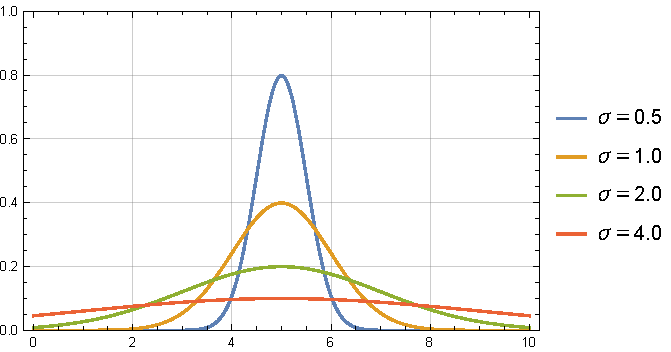
\includegraphics[scale=0.9]{Mathematica/output/GauFunc.pdf}
    \end{FigureSub}\\ \vspace{0.5cm}
    \begin{FigureSub}[正态分布的分布函数]
        \hspace{1cm}
        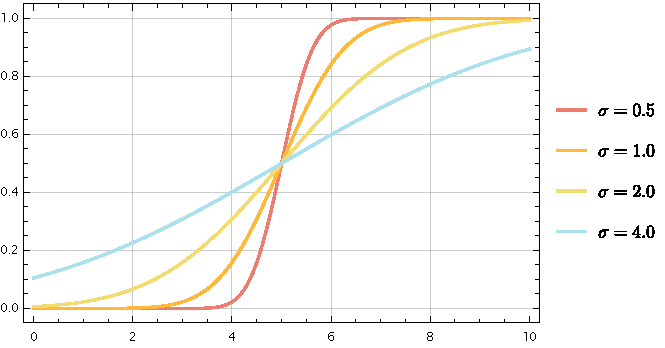
\includegraphics[scale=0.9]{Mathematica/output/GauFuncF.pdf}
    \end{FigureSub}
\end{Figure}

正态分布的归一性的证明复杂些,这需要用到高斯积分。
\begin{BoxProperty}[正态分布的归一性]
    正态分布满足归一性要求
    \begin{Equation}
        \Int[-\infty][\infty]\frac{1}{\sqrt{2\pi}\sigma}\exp[-\frac{(x-\mu)^2}{2\sigma^2}]=1
    \end{Equation}
\end{BoxProperty}

\begin{Proof}
    这需要用到高斯积分,令$t=(x-\mu)/\sqrt{2}\sigma$
    \begin{Equation}*
        \Int[-\infty][\infty]\frac{1}{\sqrt{2\pi}\sigma}\exp[-\frac{(x-\mu)^2}{2\sigma^2}]=
        \frac{1}{\sqrt{\pi}}\Int[-\infty][\infty]\e^{-t^2}\dd{t}=1\qedhere
    \end{Equation}
\end{Proof}

正态分布的分布函数很难求出,这是因为$\exp(-t^2)$的原函数无法用初等函数表示,只有上述这种计算$\exp(-t^2)$从$-\infty$到$+\infty$的特殊的定积分才能求出值,为此,引入一个特殊函数。
\begin{BoxDefinition}[误差函数]
    \uwave{误差函数}(Error Function)定义为
    \begin{Equation}
        \erf(x)=\frac{1}{\sqrt{\pi}}\Int[-x][x]\e^{-t^2}\dd{t}=\frac{2}{\sqrt{\pi}}\Int[0][x]\e^{-t^2}\dd{t}
    \end{Equation}
\end{BoxDefinition}
误差函数的图像如\xref{fig:误差函数}所示,其是一个奇函数
\begin{Figure}[误差函数]
    \hspace{1cm}
    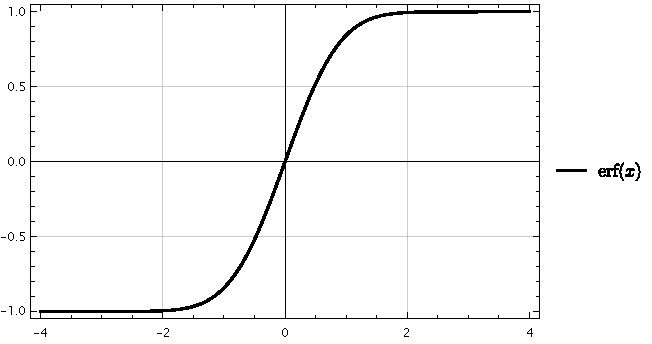
\includegraphics[scale=0.9]{Mathematica/output/erf.pdf}
\end{Figure}

这样一来,我们就至少可以形式化的写出正态函数的分布函数了。
\begin{BoxEquation}[正态分布的分布函数]
    正态分布的分布函数
    \begin{Equation}
        F(x)=\frac{1}{2}\qty[1+\erf\qty(\frac{x-\mu}{\sqrt{2}\sigma})]
    \end{Equation}
\end{BoxEquation}
\begin{Proof}
    根据\fancyref{def:正态分布},令$\tau=(\xi-\mu)/\sqrt{2}\sigma$,当$\xi=x$时有$\tau=t=(x-\mu)/\sqrt{2}\sigma$
    \begin{Equation}
        \qquad\qquad
        F(x)=\Int[-\infty][x]f(\xi)\dd{\xi}=
        \Int[-\infty][x]\frac{1}{\sqrt{2\pi}\sigma}\exp[-\frac{(\xi-\mu)^2}{2\sigma^2}]\dd{\xi}=\frac{1}{\sqrt{\pi}}\Int[-\infty][t]\e^{-\tau^2}\dd{\tau}
        \qquad\qquad
    \end{Equation}
    将积分拆分为两项,根据高斯积分和\fancyref{def:误差函数}
    \begin{Equation}
        \qquad\qquad
        F(x)=\frac{1}{\sqrt{\pi}}\qty[\Int[-\infty][0]\e^{-\tau^2}\dd{\tau}+\Int[0][x]\e^{-\tau^2}\dd{\tau}]=\frac{1}{\sqrt{\pi}}\qty[\frac{\sqrt{\pi}}{2}+\frac{1}{2}\sqrt{\pi}\erf(t)]
        \qquad\qquad
    \end{Equation}
    即
    \begin{Equation}*
        F(x)=\frac{1}{2}\qty[1+\erf\qty(\frac{x-\mu}{\sqrt{2}\sigma})]\qedhere
    \end{Equation}
\end{Proof}

实践中,我们往往需要计算$f(x)$和$F(x)$的取值,尤其是后者,考虑到它是非初等函数。但是我们不可能为所有的$\mu,\sigma$编制表格!因此,我们先定义$\mu=0$且$\sigma=1$的正态分布为标准正态分布$N(0,1)$,其概率密度和分布函数分别记为$\varphi(x)$和$\Phi(x)$,我们已经为$\Phi(x)$编制了函数表,随后证明一个简单的引理,使所有正态分布都可以通过线形变换得到标准正态分布。

\begin{BoxDefinition}[标准正态分布]
    标准正态分布是指参数满足$\mu=0$和$\sigma=1$的正态分布。

    标准正态分布的概率密度函数记为
    \begin{Equation}
        \varphi(x)=\frac{1}{\sqrt{2\pi}}\exp(-\frac{x^2}{2})
    \end{Equation}
    标准正态分布的分布函数记为
    \begin{Equation}
        \Phi(x)=\frac{1}{2}\qty[1+\erf\qty(\frac{x}{\sqrt{2}})]
    \end{Equation}
\end{BoxDefinition}

\begin{BoxLemma}[标准正态分布与正态分布]
    正态分布可以通过线性变换转化为标准正态分布,即若
    \begin{Equation}
        X\sim N(\mu,\sigma^2)
    \end{Equation}
    则有
    \begin{Equation}
        Z=(X-\mu)/\sigma\sim N(0,1)
    \end{Equation}
\end{BoxLemma}

\begin{Proof}
    我们试着来写$Z$的分布函数
    \begin{Equation}
        P\qty{Z\leq x}=
        P\qty{(X-\mu)/\sigma\leq x}=
        P\qty{X\leq\mu+\sigma x}
    \end{Equation}
    这里我们知道$X\sim N(\mu,\sigma^2)$,而根据\fancyref{def:正态分布}
    \begin{Equation}
        \qquad\qquad
        P\qty{Z\leq x}=P\qty{X\leq\mu+\sigma x}=
        \frac{1}{\sqrt{2\pi}\sigma}\Int[-\infty][\mu+\sigma x]\exp[-\frac{(\xi-\mu)^2}{2\sigma^2}]\dd{\xi}
        \qquad\qquad
    \end{Equation}
    作$\tau=(\xi-\mu)/\sigma$,而当$\xi=\mu+\sigma x$时$\tau=x$,根据\fancyref{def:标准正态分布}
    \begin{Equation}
        P\qty{Z\leq x}=\frac{1}{\sqrt{2\pi}}\Int[-\infty][x]\exp(-\frac{\tau^2}{2})\dd{\tau}=\Phi(x)
    \end{Equation}
    这就说明$Z\sim N(0,1)$,即线性变换后的$Z$服从标准正态分布。
\end{Proof}

简而言之,\xref{lem:标准正态分布与正态分布}就告诉我们,若要求正态分布在某个区间的概率
\begin{Equation}
    P\qty{x_1<X\leq x_2}=\Phi\qty(\frac{x_2-\mu}{\sigma})-\Phi\qty(\frac{x_1-\mu}{\sigma})
\end{Equation}
由此,根据$\Phi(x)$的函数表,我们很容易确定出对于服从正态分布的随机变量$X$,其落在以参数$\mu$为中心,半径为$1\sigma, 2\sigma, 3\sigma$的区间中的概率(即钟形曲线下的面积),如\xref{tab:正态分布的概率特征}所示。
\begin{Table}[正态分布的概率特征]{llr}
<范围&表达式&概率\\>
$P\qty{\mu-1\sigma<X<\mu+1\sigma}$&
$\Phi(1)-\Phi(-1)=2\Phi(1)$&$0.6826$\\
$P\qty{\mu-2\sigma<X<\mu+2\sigma}$&
$\Phi(2)-\Phi(-2)=2\Phi(2)$&$0.9544$\\
$P\qty{\mu-2\sigma<X<\mu+2\sigma}$&
$\Phi(2)-\Phi(-2)=2\Phi(2)$&$0.9974$\\
\end{Table}

或者,如\xref{fig:正态分布的概率特征}所示
\begin{Figure}[正态分布的概率特征]
    \includegraphics{build/Chapter02C_01.fig.pdf}
\end{Figure}

总之,我们看到,尽管正态分布的变量的取值范围是$(-\infty,\infty)$,但它的值落在$3\sigma$区间内的机会是很大的,概率高达$99.74\%$,这也就是我们常说的$3\sigma$法则。类似的例子出现在大学物理实验中,那时我们使用的不确定度对应的置信度为$95.44\%$,对应的置信区间即$2\sigma$区间。

\begin{BoxDefinition}[标准正态分布的上分位数]
    设随机变量$X\sim N(0,1)$,若$z_\alpha$满足条件
    \begin{Equation}
        P(X>z_\alpha)=\alpha
    \end{Equation}
    则称$z_\alpha$为标准正态分布的\uwave{上$\alpha$分位数}。
\end{BoxDefinition}
如\xref{fig:正态分布的上分位数}所示,所谓上$\alpha$分位数$z_\alpha$,即是指概率要当$x$大于多少时才能降低到$\alpha$以内。

\begin{Figure}[正态分布的上分位数]
    \includegraphics{build/Chapter02C_02.fig.pdf}
\end{Figure}

在\xref{tab:正态分布的上分位数}中,我们列出了几个常用的$z_\alpha$值
\begin{Table}[正态分布的上分位数]{cc}
<$\alpha$&$z_\alpha$\\>
0.100&1.282\\
0.050&1.645\\
0.025&1.960\\
0.010&2.326\\
0.005&2.576\\
0.001&3.090\\
\end{Table}

正态分布在概率论与数理统计中起着特别版重要的作用,之后我们会更深刻的认识这一点。